\subsection{Interface}

\begin{flushleft}
Pour inclure l'extension dans l'interface, j'ai dû changer 3 pages.
\end{flushleft}

\begin{enumerate}[-]
\item Add a wallet
\item Name (wallet)
\item Consumptions
\end{enumerate}

\begin{flushleft}
Suivant les explications de la base de données, le client devra entrer plus d'informations dans la fenêtre \textbf{Add a wallet} et nous pouvons également les afficher dans \textbf{Name (wallet)} vu que le client souhaite voir toutes les informations du portefeuille dans celui-ci.
\end{flushleft}

\begin{flushleft}
Dans le cas de \textbf{Consumptions}, j'ai d'abord rajouté trois boutons dans le bas de page. Ils représentent les différents modes, c'est-à-dire:
\end{flushleft}

\begin{enumerate}[-]
\item Voir sa consommation \textbf{Just see}
\item Comparer ses consommations \textbf{Compare}
\item Comparer sa consommation avec quelqu'un d'autre (simulation) \textbf{Compare with other}
\end{enumerate}

\begin{flushleft}
Finalement, j'ai placé un tableau en plus pour le cas où l'on veut comparer des données. Comme vous pouvez le voir, il y a également deux boutons au-dessus de chaque tableau qui permettent de choisir si l'on veut voir les données pures ou les statistiques.
\end{flushleft}

\begin{figure}[h]
\centering
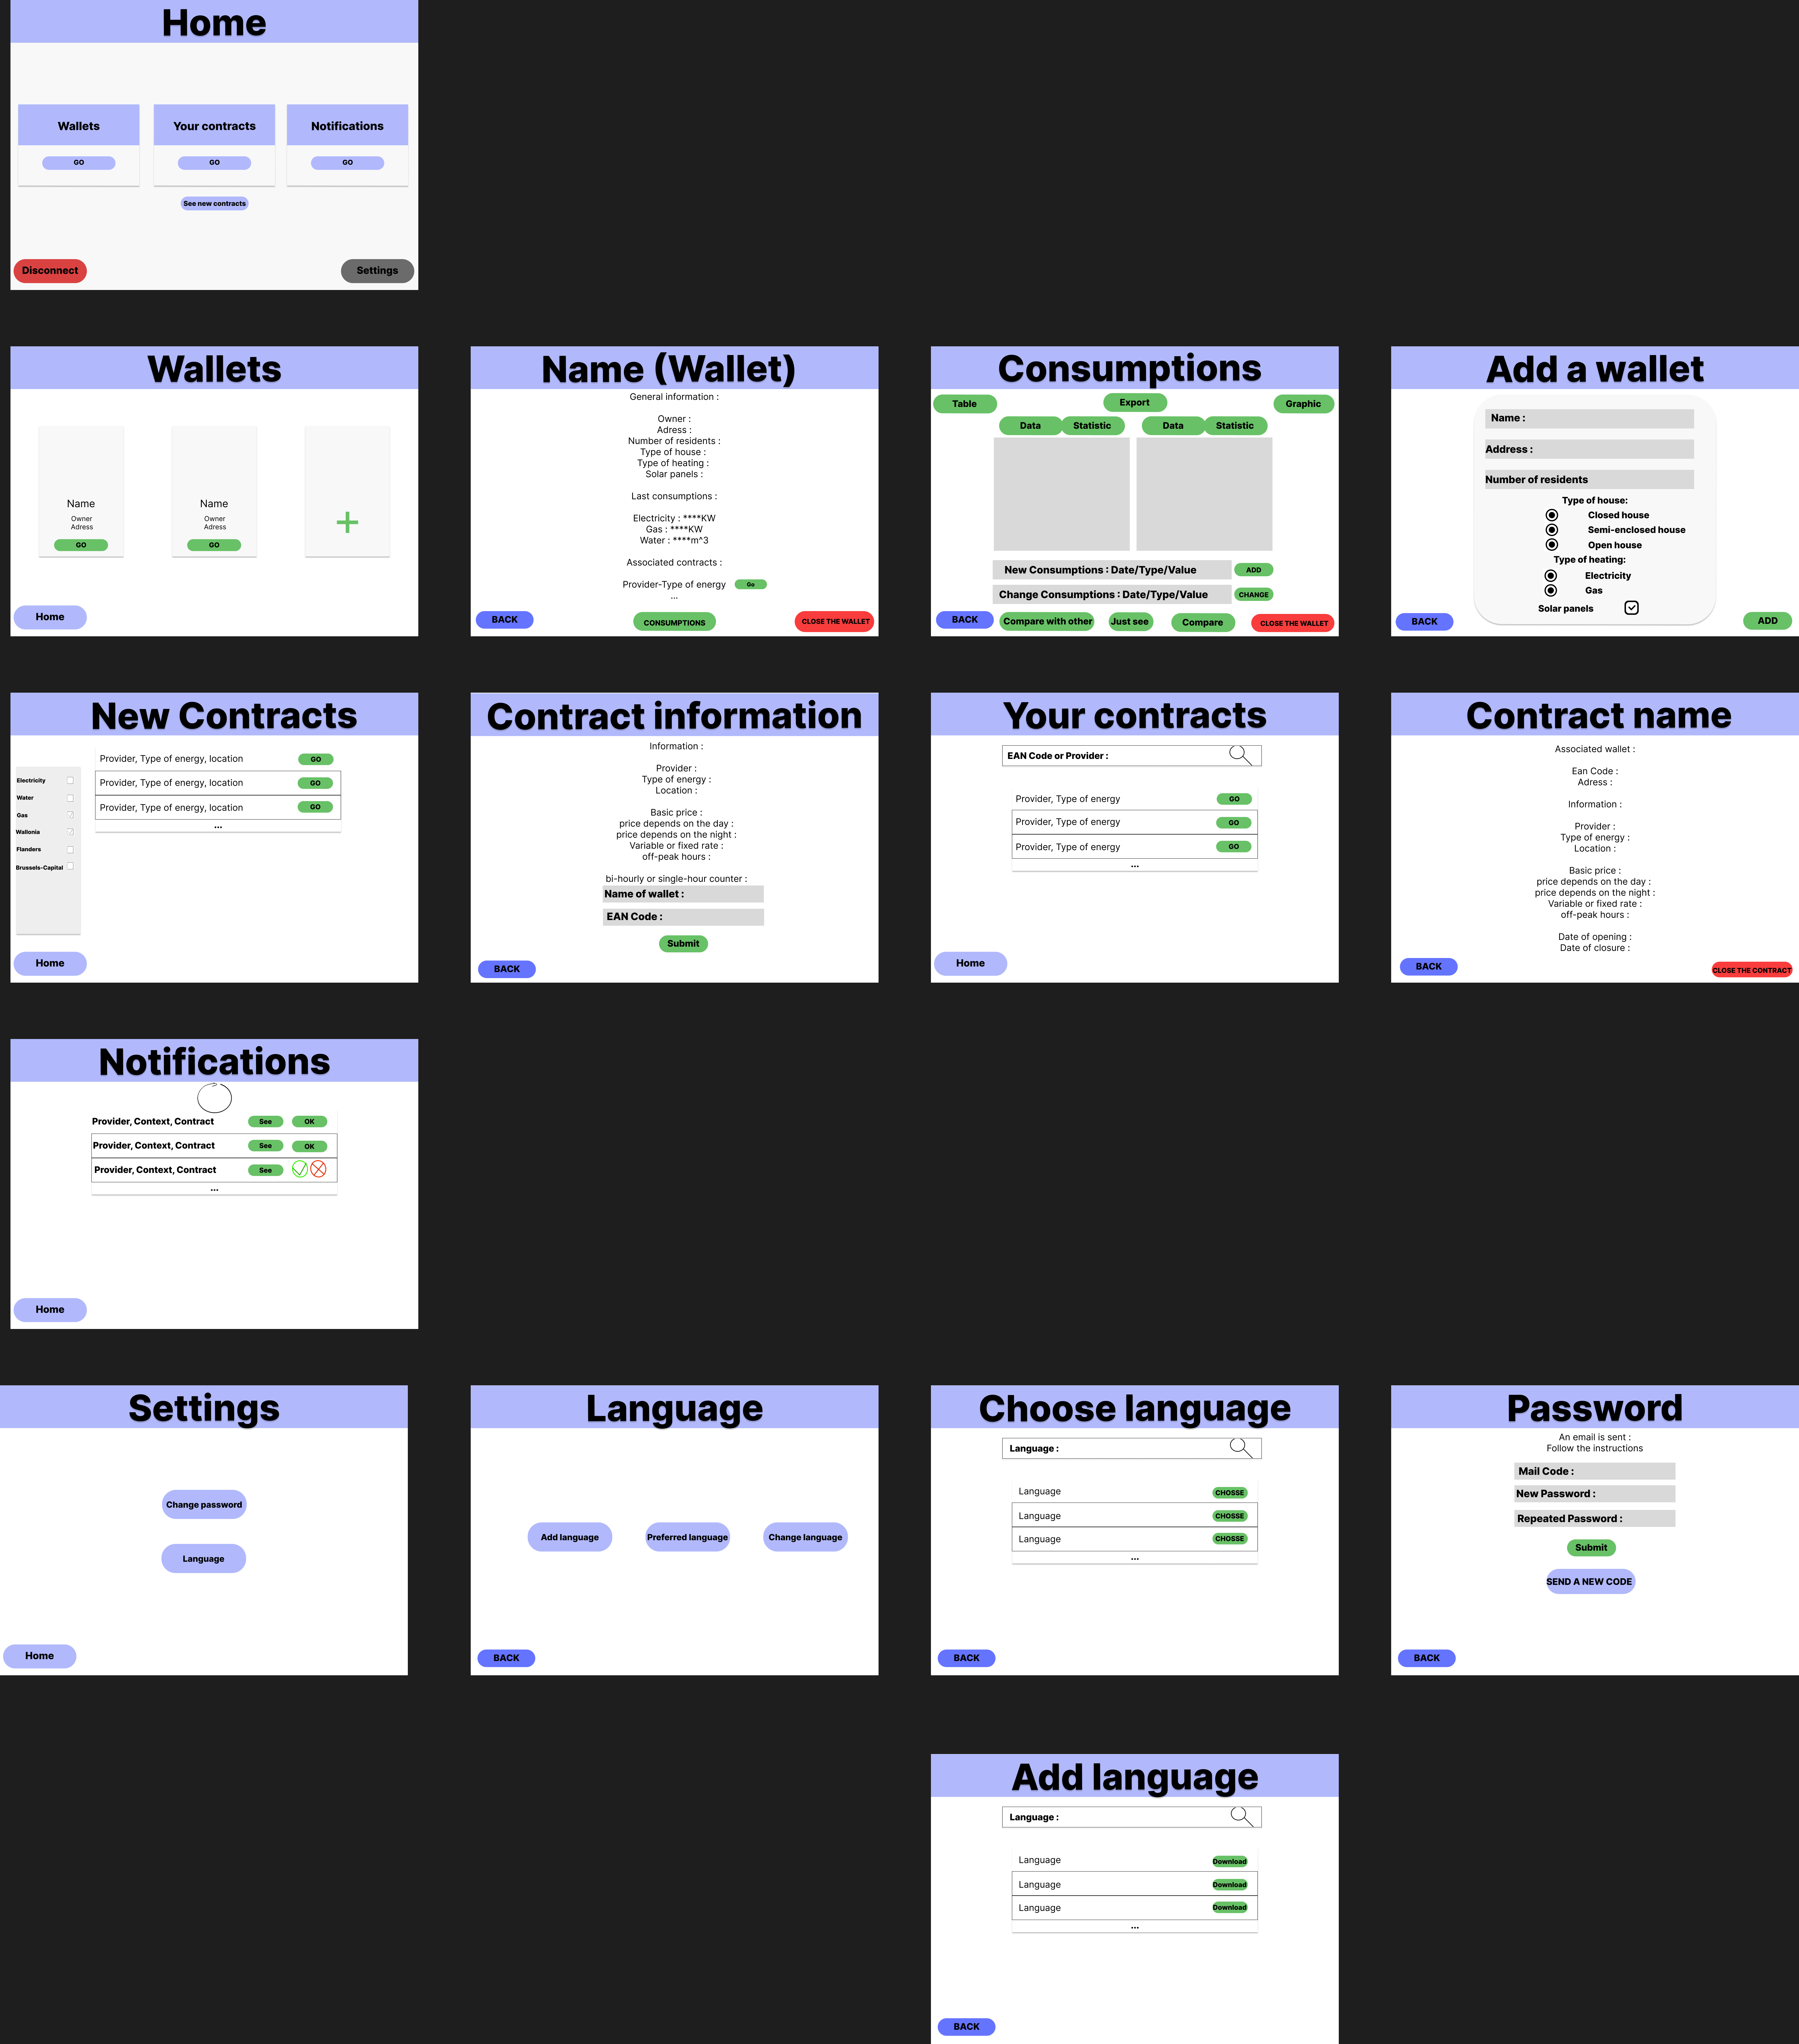
\includegraphics[width=1.3\textwidth]{extension-adrien/Interface/img/interface.png}
\end{figure}
